%%%%%%%%%%%%%%%%%%%%%%%%%%%%%%%%%%%%%%%%%
% University Assignment Title Page
% LaTeX Template
% Version 1.0 (27/12/12)
%
% This template has been downloaded from:
% http:\\www.LaTeXTemplates.com
%
% Original author:
% WikiBooks (http:\\en.wikibooks.org/wiki/LaTeX/Title_Creation)
%
% License:
% CC BY-NC-SA 3.0 (http:\\creativecommons.org/licenses/by-nc-sa/3.0/)
% %%%%%%%%%%%%%%%%%%%%%%%%%%%%%%%%%%%%%%%%
\documentclass[12pt]{article}
\usepackage[hidelinks]{hyperref}
\hypersetup{linktoc=all}
\usepackage{xcolor}

\usepackage{float}

\usepackage{graphicx}
\graphicspath{{Resources/}}

\begin{document}
\sloppy

\begin{titlepage}

\newcommand{\HRule}{\rule{\linewidth}{0.5mm}} % Defines a new command for the
%horizontal lines, change thickness heReve

\center % Center everything on the page

%----------------------------------------------------------------------------------------
%	HEADING SECTIONS
%----------------------------------------------------------------------------------------

\textsc{\LARGE McMaster University}\\[1.5cm] % Name of your university/college
\textsc{\Large Software Project Management}\\[0.5cm] % Major heading such as course name
\textsc{\large SFWR ENG 3XA3}\\[0.5cm] % Minor heading such as course title

%----------------------------------------------------------------------------------------
%	TITLE SECTION
%----------------------------------------------------------------------------------------

\HRule \\[0.4cm]
{ \huge \bfseries Requirements Document}\\[0.4cm] % Title of your document
\HRule \\[1.5cm]

%----------------------------------------------------------------------------------------
%	AUTHOR SECTION
%----------------------------------------------------------------------------------------



% If you don't want a supervisor, uncomment the two lines below and remove the section above
\Large \emph{Authors:}\\
Mohammad \textsc{Naveed} \textbf{1332196} \\ % Your name
Josh \textsc{Voskamp} \textbf{1319352} \\
Stephan \textsc{Arulthasan} \textbf{1308004} \\[3cm]
%----------------------------------------------------------------------------------------
%	DATE SECTION
%----------------------------------------------------------------------------------------

{\large \today}\\[3cm] % Date, change the \today to a set date if you want to be precise

%----------------------------------------------------------------------------------------
%	LOGO SECTION
%----------------------------------------------------------------------------------------

%\includegraphics{Logo}\\[1cm] % Include a department/university logo - this will require the graphicx package

%----------------------------------------------------------------------------------------

\vfill % Fill the rest of the page with whitespace

\end{titlepage}

\newpage
\tableofcontents
\newpage
\listoftables
\addcontentsline{toc}{section}{List of Tables}
\newpage
\listoffigures
\addcontentsline{toc}{section}{List of Figures}
\newpage

\section*{Revision History}
\addcontentsline{toc}{section}{Revision History}
\begin{table}[H]
	\centering
	\begin{tabular}{ | p{2cm} |  p{2cm} | p{5cm} | p{3.8cm} |}
		\hline
		Rev. No. & Rev. Date & Description & Author \\\hline
		0 & Oct 5 2015 & Created Document & Mohammad Naveed \\\hline
		0 & Oct 5 2015 & Added Off the Shelf Software & Josh Voskamp \\\hline
		0 & Oct 7 2015 & Added Functional Requirements & Stephan Arulthasan\\\hline
		0 & Oct 7 2015 & Improve Formatting & Josh Voskamp \\\hline
		0 & Oct 9 2015 & Improved Functional Requirements & Stephan Arulthasan \\\hline
		0 & Oct 9 2015 & Added Non-Functional Requirements & Mohammad Naveed \\\hline
		0 & Oct 9 2015 & Create Project Issues & Josh Voskamp \\\hline
		0 & Oct 9 2015 & Add to Project Issues & Mohammad Naveed \\\hline
		0 & Oct 9 2015 & Complete Project Issues & Stephan Arulthasan \\\hline
		0 & Oct 9 2015 & Finalize Requirements Documentation & Josh Voskamp \\\hline
        \color{red} 1 &\color{red} Dec 3 2015 &\color{red} Add Client, Risks, Context Diagram, Input and Output, Activity Diagram &\color{red} Josh Voskamp \\\hline
	\end{tabular}
	\caption{Revision History}
\end{table}
\newpage

\section{Purpose of the Project}
\subsection{What is the problem being solved?}
\par\indent\indent It is commonly known that technology, although serving countless purposes, is a large source of distraction to many people. More specifically, online applications, although highly entertaining and addicting, are very limited in cognitive stimulation. This is highly problematic as we are enabling a culture of absent minded technological engagement.
\subsection{Why is this an Important Problem?}
\par\indent\indent According to Jane McGonigal, a well known and world renowned game designer; we spend 3 billion hours a week playing video games. That is a lot of time that many people argue could be spent better, and that is what 2048 aims to accomplish. More and more people are playing video games everyday and 2048 is a fun and challenging game that tests the users' mathematical as well as their spatial intelligence. This allows 2048 to be fun, yet still be brain enhancing. Since the target audience for this game is so large, we can take advantage of this by providing users an option to spend their gaming time in a way thats beneficial mentally while still being entertained.
\subsection{Context of the problem}
\par\indent\indent Everyone experiences idle time in their day; this could be waiting for an appointment, a class, a bus or for friends. This game is intended to appeal to everyone looking for a more entertaining way to spend their idle time. The complexity of the game is meant to provide a challenge so that the user does not feel like they are wasting time, but using their time constructively. The game will be playable on all of the three major operating systems, OSX, Windows, and Linux with possible future expansion to mobile devices.

\section{Stakeholders}
\subsection{\color{red}Client}
\begin{itemize}
    \color{red}
    \item Dr. Spencer Smith
    \item Peng Li
\end{itemize}
\subsection{Customer}
\begin{itemize}
    \item Gamer
\end{itemize}
\subsection{Other Stakeholders}
\begin{itemize}
    \item Developers and Testers
\end{itemize}

\section{Users of the Product}
\subsection{Hands-On Users of the Product}
\par\indent\indent Any person with any computer running the Java Runtime Environment can use our game to relieve stress and build on their mathematical and spatial intelligence.
\subsection{Priorities assigned to Users}
\textbf{Primary Users:} Windows, Mac OSX, and LINUX users\\
\textbf{Secondary Users:} Developers, testers and supervisors

\subsection{User Participation}
\begin{itemize}
    \item User just has to play the game to participate
\end{itemize}
\subsection{Maintainence Users and Testers}
\begin{itemize}
    \item Developers/Testers
\end{itemize}

\section{Project Constraints}
\subsection{Mandated Constraints}
\textbf{Description:} The product shall operate using Windows, Mac OSX and LINUX\\
\textbf{Rationale:} Users do not want to change operating systems just for the game and it will be more convenient for them.\\
\textbf{Description:} Product should be easy to use for people over the age
of 10\\
\textbf{Rationale:} The product does require a certain level of mathematical and spatial intelligence which is why users under 10 years of age may find it difficult to use.
\subsection{Off the Shelf Software}
\par\indent\indent The open source project that is being improved can be found at: \\ \url{https://github.com/bulenkov/2048}\\
This implementation of 2048 is based off the original 2048 game created by Gabriele Cirulli which was also based off a small clone of 1024. https://github.com/gabrielecirulli/2048.
\subsection{Anticipated Workplace Enviroment}
This application is expected to be used at home, in the workplace, at school, and in the public.\\
\subsection{Schedule Constraints}
Requirements Document Revision 0	\hfill	October 9 \\
Proof of Concept Demonstration \hfill		October 26-28 \\
Final Demonstration \hfill				November 30 - December 4 \\

\section{Functional Requirements}
\subsection{Scope of the Project}
Everyone experiences idle time in their day; this could be waiting for an appointment, a class, a bus or for friends. That is a lot of time that many people argue could be spent better, and that is what 2048 aims to accomplish. 2048 is a game in which the user uses the arrow keys to combine alike tiles in an attempt to reach the "2048" tile.\\

\subsection{\color{red}Context of the Work}

\begin{figure}[H]
    \color{red}
	\centering
	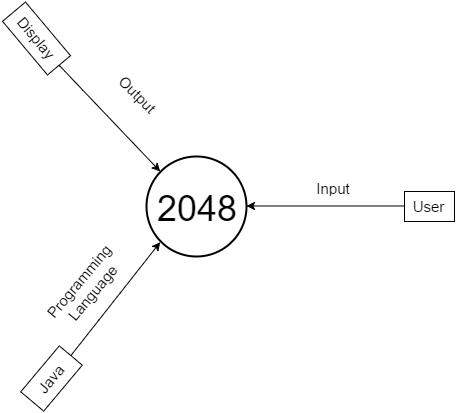
\includegraphics[width = 10cm]{context_diagram}
	\caption{\textcolor{red}{Context Diagram}}
	\label{Context Diagram}
\end{figure}

\subsection{\color{red}Product Uses Case}
\begin{figure}[H]%used figure to keep this whole section together
    \color{red}
	\textbf{Product Use Case Name:} Move\\
	\textbf{Trigger:} User Access\\
	\textbf{Preconditions: } None\\
	\textbf{Interested Stakeholders: } Client and Gamer\\
	\begin{figure}[H]%the figure that actually contains an image
		\color{red}
		\centering
		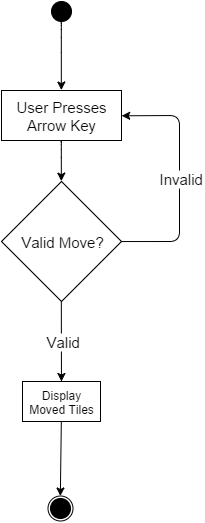
\includegraphics[height = 12cm]{activity_diagram}
		\caption{\textcolor{red}{Activity Diagram for Move}}
		\label{Activity Diagram for Move}
	\end{figure}
\end{figure}

\subsection{\color{red}Input and Output}
\begin{table}[H]
    \color{red}
	\centering
	\begin{tabular}{ | p{5cm} |  p{5cm} | p{5cm} |}\hline
        \textbf{Event Name} & \textbf{Input and Output} & \textbf{Summary} \\\hline
        Move Left & Left Arrowkey(in) & Tiles Shift Left \\\hline
        Move Right & Right Arrowkey(in) & Tiles Shift Right \\\hline
        Move Up & Up Arrowkey(in) & Tiles Shift Up \\\hline
        Move Down & Down Arrowkey(in) & Tiles Shift Down \\\hline
        Restart & ESC(in) & Game Restarts \\\hline
	\end{tabular}
	\caption{\textcolor{red}{Input and Output Table}}
\end{table}
\subsection{Functional and Data Requirements}
\textbf {Requirement \#:1} \\\\
\textbf {Description:} The user must be able to start a game.\\
\textbf {Rational:} In order for the player to play the game, it has to initialize first.\\
\textbf {Fit Criterion:} User successively starts game so they can play. \\\\

\textbf {Requirement \#:2}  \\\\
\textbf {Description:} The user must be able to restart the game.\\
\textbf {Rational:}The user may want to restart if they made a bad move or have already won or lost the game. \\
\textbf {Fit Criterion:}Users successfully restarts the game. \\\\

\textbf {Requirement \#:3} \\\\
\textbf {Description:} The user must be able to exit the game.\\
\textbf {Rational:} The user may want to exit the session at any time.\\
\textbf {Fit Criterion:} User successfully exits game. \\\\

\textbf {Requirement \#:4} \\\\
\textbf {Description:}The user must be able to make valid moves. \\
\textbf {Rational:} In order to play and win the game, the user must be able to move the tiles around. \\
\textbf {Fit Criterion:}User successfully makes a valid move within the gameboard, where the tiles join correctly and score counter increases by the value created. \\\\

\textbf {Requirement \#:5}  \\\\
\textbf {Description:} The user must be able to win the game.\\
\textbf {Rational:} The player is working towards making the 2048 tile. \\
\textbf {Fit Criterion:} User successfully makes the 2048 tile and the game ends. \\\\

\textbf {Requirement \#:6} \\\\
\textbf {Description:}The user must be able to lose the game. \\
\textbf {Rational:} It is possible to make a bad sequence of moves in the game so that all the tiles are filled and no more moves can be created.\\
\textbf {Fit Criterion:} The user fills up all the tile spaces and the game ends.\\\\

\textbf {Requirement \#:7}  \\\\
\textbf {Description:} The product must display the game score.\\
\textbf {Rational:} The user will be able to rank themselves against other players and try to beat their own high score.\\
\textbf {Fit Criterion:} Product successfully displays score based on moves made by user.\\\\

\textbf {Requirement \#:8}  \\\\
\textbf {Description:} The product must notify the user if they win or lose.\\
\textbf {Rational:} The user must be able to tell if they successfully win the game. Also, the tiles on the screen may be filled up but that doesn't necessarily mean they lost because there can be moves available. \\
\textbf {Fit Criterion:} The game displays a win notification when the user reaches the 2048 tile and a lose notification when the user fills up all the tile spaces with no moves left. \\\\

\section{Non-Functional Requirements}

\subsection{Look \& Feel Requirements}
\begin{itemize}
    \item Appearance Requirements
    \begin{itemize}
        \item Board size must be 4x4
        \item The interface must be intuitive
    \end{itemize}
\end{itemize}
\subsection{Usability Requirements}
\begin{itemize}
    \item Ease of use Requirements
    \begin{itemize}
        \item Product shall be easy to use for anyone who is older than the age of 10
    \end{itemize}
    \item Personalization and Internationalization Requirements
    \begin{itemize}
        \item N/A
    \end{itemize}
    \item Ease of Learning of Requirements
    \begin{itemize}
        \item The product shall be easy to learn for anyone who is older than the age of 10
    \end{itemize}
\end{itemize}
\subsection{Performance Requirements}
\begin{itemize}
    \item Speed requirements
    \begin{itemize}
        \item The game must start in under 2 seconds
        \item Any interaction with the user and the product during gameplay must have a maximum response time of 2 seconds
    \end{itemize}
    \item{Precision Requirements}
    \begin{itemize}
        \item All values on the tiles must be integers
        \item The value of the smallest tile must be 2
        \item The value of the largest tile must be 2048
        \item The value on all tiles must be a multiple of 2
    \end{itemize}
    \item{Reliability \& Availability Requirements}
    \begin{itemize}
        \item The product shall be available for use 24 hours a day for 365 days of the year
    \end{itemize}
    \item{Safety Critical Requirements}
    \begin{itemize}
        \item \textcolor{red}{This game must not hurt anyone}
    \end{itemize}
    \item{Capacity Requirements}
    \begin{itemize}
        \item The product shall cater to 1 user on the machine
    \end{itemize}
\end{itemize}

\subsection{Operational Requirements}
\begin{itemize}
    \item Expected Physical Environment
    \begin{itemize}
        \item The product is to be used by gamers at home, in the workplace, at school, and in the public
    \end{itemize}
    \item Expected Technological Environment
    \begin{itemize}
        \item The product shall be available on LINUX, Mac OSX, and Windows operating systems
        \item The environment must have the Java Runtime Environment (JRE)
    \end{itemize}
    \item Partner Applications
    \begin{itemize}
        \item N/A
    \end{itemize}
\end{itemize}

\subsection{Maintainability and Support Requirements}
    \begin{itemize}
        \item Maintenance Requirements
    \begin{itemize}
        \item Make it easy to fix any potential bugs in the code
    \end{itemize}
    \item Supportability Requirements
    \begin{itemize}
        \item The product will not be supported, however the source code will be available for examination or enhancement.
    \end{itemize}
    \item Adaptability Requirements
    \begin{itemize}
        \item The product is expected to run on LINUX, Mac OSX, and Windows operating systems
    \end{itemize}
\end{itemize}

\subsection{Security Requirements}
\begin{itemize}
    \item N/A
\end{itemize}

\subsection{Cultural Requirements}
\begin{itemize}
    \item The product shall not use icons that could be considered offensive in any of our market countries.
\end{itemize}

\subsection{Compliance Requirements}
\begin{itemize}
    \item N/A
\end{itemize}

\section{Project Issues}
\subsection{Open Issues}
\begin{itemize}
	\item Creating a GUI compatible with various screen resolutions
	\item Animation for the sliding of the tiles
	\item Add a FAQ option
\end{itemize}

\subsection{Off-the-Shelf Solutions}
\begin{itemize}
	\item \url{https://github.com/bulenkov/2048} The Open-source Java project being improved.
	\item \url{https://github.com/gabrielecirulli/2048} The Original Open-source 	project for the game 2048, It was originally implemented in JavaScript.
\end{itemize}

\subsection{New Problems}
\subsubsection{Effects on the Current Environment}
N/A
\subsubsection{Effects on the Installed Systems}
N/A
\subsubsection{Potential User Problems}
N/A
\subsubsection{Limitations in the Anticipated Implementation Environment That
May Inhibit the New Product}
N/A
\subsubsection{Follow-Up Problems}
N/A
\subsection{Costs}
There are no direct monetary costs associated with this project, but about half a year of development time will be required.\\

\subsection{User Documentation and Training}
User's will provided with information on program use via a FAQ option which, when selected, will open a dialog box detailing general functionality of the program. Beyond the help document, user?s familiar with casual computer use should require no further training.\\

\subsection{Tasks}
\begin{itemize}
	\item Revise requirements document.
	\item Create a test plan.
	\item Demonstrate a proof of concept.
	\item Draw up design documents.
	\item Revision 0 project demonstration.
	\item Create a user guide for the project.
	\item Write up a test report
	\item Final revision project demonstration.
	\item Write final revisions to documentation.
\end{itemize}

\subsection{\color{red}{Risks}}
\begin{itemize}
    \color{red}
    \item Team members not doing their assigned tasks
    \item Team members not following deadlines set by the team, or client
    \item Project not compiling for the Professor or TA
\end{itemize}

\subsection{Waiting Room}
There are no plans to introduce new releases of this product. If that were to change, new features would include an animated GUI and an online high score list.

\subsection{Ideas for Solutions}
\begin{itemize}
	\item Use Java Swing and AWT for GUI development
\end{itemize}

\end{document}
